% main.tex
\documentclass[12pt]{article}

\usepackage[margin=1in]{geometry}
\usepackage{natbib}
\usepackage{hyperref}
\hypersetup{
  colorlinks=true,
  linkcolor=blue,
  filecolor=magenta,
  citecolor=blue,
  urlcolor=cyan,
  pdftitle={How to Study Boundary Phenomena},
  pdfpagemode=FullScreen,
}
\usepackage[T1]{fontenc}
\usepackage[utf8]{inputenc}
\usepackage{amsmath}
\usepackage{graphicx}
\usepackage{tipa}
\usepackage{setspace}
\usepackage{booktabs}
\usepackage{ulem}

\title{Language as a Stack of Homeostatic Property-Cluster Kinds: From Phonemes to Constructions}
\author{Brett Reynolds}
\date{}

\begin{document}
\maketitle
\doublespacing

\begin{abstract}
\noindent Categories in language are stable enough to support reliable inference but flexible enough to drift, diversify, and admit exceptions. I argue that many linguistic categories~-- phonemes, lexemes, and language-internal constructions~-- are \textsc{homeostatic property-cluster} (HPC) kinds: probabilistic clusters of articulatory, acoustic, semantic, and distributional properties stabilized by identifiable mechanisms at biological, cognitive-developmental, and sociocultural levels. Building on Miller's (\citeyear{Miller2021WordsSpeciesKinds}) account of words as HPCs, which rejects essence-based individuation in favor of mechanism-indexed clusters, and on recent evidence that phonemes function as culturally maintained cognitive tools, I generalize the HPC template across linguistic levels and supply operational diagnostics and compact case studies. The diagnostics are (i) a projectibility test: tokens of a proposed kind support out-of-sample inferences about form/meaning/distribution; and (ii) a homeostasis test: specific stabilizers can be named and their property covariance shown. I demonstrate these with (A) phoneme typology (inventory ridgelines by family and the probability of /y/ increasing with vowel-inventory size), (B) a word-level diachrony showing distributional ``cluster cohesion'' under semantic drift, and (C) an English construction (\textit{let alone}), with cue bundling and cross-corpus replication. I also delimit non-HPCs: one-off items (nonce coinages), analyst-level macro-categories (e.g., cross-linguistic ``resultative'' as a single kind), and negative/complement classes. The result is a general method for deciding when a linguistic category earns kindhood by HPC lights, why some categories travel well across speakers and time, and where category proposals fail.
\end{abstract}

\section{Introduction}
Language presents a familiar problem for cognitive science: the categories we rely on to speak and understand are stable enough to underwrite reliable inference but flexible enough to drift and diversify. Consider how the phoneme /r/ varies across English dialects but remains recognizable, or how the word \textit{awful} drifted from `awe-inspiring' to `terrible' while keeping its identity. An attractive middle ground for understanding such categories~-- originating in Boyd's account of \textsc{homeostatic property-cluster} (HPC) kinds~-- offers a way to reconcile stability with change \citep{Boyd1991Enthusiasm,Boyd1999Homeostasis}\footnote{For the first explicit HPC formulation (applied to moral terms), see \citet[§3.8]{Boyd1988MoralRealist}. For an explicit allowance that social mechanisms can underwrite homeostasis, see \citet{Boyd2000Workmanship}.}.

A homeostatic property cluster treats a category as a family of properties kept together by mechanisms (biophysical, developmental, social) strongly enough to support induction, without positing a single essence. Think of biological species: robins share characteristic features~-- size, coloration, song patterns, nesting behavior~-- not because of an essential `robin-ness' but because developmental programs, ecological pressures, and reproductive isolation keep these traits correlated generation after generation. Boyd's insight is that many scientific and social categories work similarly: they are probabilistic clusters stabilized by mechanisms that keep enough of the cluster together for inductive use. On this understanding, I treat phonemes, words, and language-internal constructions (e.g., English \textit{let alone}) as a posteriori kinds maintained by identifiable stabilizers.

For words, \citet{Miller2021WordsSpeciesKinds} develops this stance, rejecting essence-based individuation in favor of mechanism-indexed clusters that are historically delimited and population-relative. On this view, word-kinds earn their status because internal (cognitive) and external (normative) mechanisms sustain covarying properties~-- pronunciation, orthography, meaning, distribution~-- so that speakers can project from attested tokens to new ones. The word \textit{dog}, for instance, maintains its identity not through a platonic essence but because spelling conventions, pronunciation norms, semantic associations, and syntactic patterns travel together, stabilized by frequency of use, literacy education, and community practice.

At the phonological level, recent work argues that phonemes are culturally maintained \textsc{cognitive tools} anchored in articulatory and auditory constraints. Two quantitative signatures exemplify the sort of measurable ``homeostasis'' HPC requires: family-wise \textsc{ridgelines} of inventory sizes (showing most languages cluster roughly between 20 and 50 segments across unrelated language families; see Figure \ref{fig:ridgelines}), and a scaling curve in which the probability that a language includes /y/ rises with vowel-inventory size, while /i/ remains common even in small systems. Both patterns are presented with explicit methodological detail and tied to biophysical and efficiency pressures, drawing on data from PHOIBLE \citep{MoranEtAl2019PHOIBLE}~-- an openly available database of segmental phoneme inventories for over 2{,}000 languages worldwide~-- and a compact checklist of tool criteria summarizes the stabilizers involved \citep[Fig.\,1 p.\,4; Fig.\,2 p.\,7; Table\,1 p.\,14]{Ekstrom2025PhonemeTool}. These are precisely the ingredients HPC seeks: projectible distributions and identifiable stabilizing mechanisms.

This article proposes a general, testable program: many linguistic categories~-- phonemes, lexemes, and language-internal constructions~-- are HPC kinds. The claim is operational, not merely analogical. I introduce two diagnostics and apply them across levels with compact, reproducible case studies, alongside a principled failure taxonomy that blocks over-generalization.

Diagnostic 1: \textsc{Projectibility}. A proposed category is projectible if tokens support reliable out-of-sample inference about form, meaning, or distribution. This can be quantified with cross-corpus replication, held-out prediction, or cluster-cohesion under temporal or register shifts.

Diagnostic 2: \textsc{Homeostasis}. A proposed category is homeostatic if its property cluster can be tied to specific stabilizers and if the expected covariance among properties can be demonstrated. Stabilizers are mechanisms that actively maintain the correlation among properties. In the case of vowels, for instance, they operate at three levels: biophysical attractors (e.g., quantal stability regions in the vocal tract that make /i/ robust; dispersion pressures that keep vowels maximally distinct), acquisition dynamics (e.g., perceptual magnets that pull variable tokens toward prototypes; sensorimotor adaptation that aligns production and perception), and sociocultural norms (e.g., local performance standards for `correct' pronunciation; entrenchment through repeated use).

The first case study revisits the phoneme level using the PHOIBLE database introduced above, but focuses on observable patterns rather than re-deriving articulatory physiology. I examine two signatures: how inventory sizes cluster by language family (visualized as ridgelines), and how the probability of finding /y/ in a language increases with the size of its vowel inventory. These patterns survive robustness checks like sampling one language per subfamily. The HPC reading is straightforward: the tight clustering within families demonstrates projectibility (new languages behave like their relatives), while the known mechanisms~-- quantal stability, dispersion, developmental tuning, and community norms~-- provide the homeostatic foundation \citep{Ekstrom2025PhonemeTool}.

The second case study turns to words. Building on \citet{Miller2021WordsSpeciesKinds}, I track how a single lexeme's meaning changes over time (e.g., how \textit{awful} drifted from positive to negative) while examining whether its contextual patterns~-- what words appear near it~-- remain coherent enough that a model trained on earlier decades can still identify the word in later ones. This demonstrates projectibility empirically. The homeostasis comes from multiple forces: entrenchment through repeated use and norm-guided conventions ensure that even as meanings shift, the word's spelling, pronunciation, and core distributional patterns stay bundled together at usable levels.

The third case study treats an English construction, \textit{let alone}, as a language-internal HPC kind. This construction (as in \textit{I can't afford coffee, \uline{let alone} dinner}) signals that the second item is even less likely than the first. Its identifying features~-- the phrase itself, parallel syntax between the contrasted items, and negative context~-- work together as a cue bundle that remains stable across different text collections. I test projectibility by training a model to recognize the construction in one corpus and seeing if it succeeds in another. The stabilizers that maintain this pattern include its frequency of use, the redundancy of its multiple cues (if one fails, others compensate), and normative enforcement through editorial practices that correct malformed instances.

Equally important are the failure cases~-- categories that don't qualify as HPC kinds. Some proposals are too thin: one-off items (like nonce coinages such as \textit{bromance} before it caught on), speech errors that blend words together, and children's overregularizations (\textit{goed} for `went') lack the stabilizers that would make them predictable beyond their immediate context. Others are too fat: when typologists group together all ``resultative'' constructions across languages, or all ``ditransitive'' patterns, they're pooling structures maintained by completely different mechanisms in each language. Since the stabilizing mechanisms are local to each language, the cross-linguistic umbrella isn't a single HPC kind. Finally, negative or complement classes (e.g., ``all ungrammatical strings'') are defined by what they're not, rather than by shared properties held together by identifiable mechanisms. The discipline here is mechanism-first, in line with the word-kinds program \citep{Miller2021WordsSpeciesKinds}.

The framework yields predictions and disconfirmers. A perturbation prediction: weakening a stabilizer (e.g., lowering frequency or impoverishing input) will reduce cluster covariance before norms re-stabilize~-- a pattern testable under register shifts or in learner corpora. A scaling prediction: rarer but quantally robust members (e.g., /y/ in the vowel space) become more probable as system size grows; analogously, low-frequency constructional variants should be more prevalent in larger constructicons. Both predictions borrow directly from the phoneme results \citep[Fig.\,2 p.\,7]{Ekstrom2025PhonemeTool} and extend them to higher levels.

In sum, properly operationalized HPC naturalizes linguistic ontology for cognitive science. It tells us when a category is the right sort of thing to underwrite inference, what keeps it stable enough, and how it can change. At the phoneme level, the ridgeline and scaling patterns already instantiate homeostasis under constraint; at the word and construction levels, analogous signatures can be demonstrated with standard corpus methods. The result isn't that everything is an HPC, but that many linguistic categories pass a disciplined test~-- and some don't \citep{Miller2021WordsSpeciesKinds,Ekstrom2025PhonemeTool}.

\section{Framework and diagnostics}\label{sec:framework}

The claim that linguistic categories are HPC kinds is ontological in spirit but have to be cashed out operationally. On the Boydian view, kinds are a posteriori and population–time relative: they are groupings whose members share a family of properties tightly enough for inductive use because there are mechanisms that, in fact, keep enough of those properties together \citep{Boyd1991Enthusiasm,Boyd1999Homeostasis}. Boyd first articulates the \textsc{HPC} template for moral terms \citep[§3.8]{Boyd1988MoralRealist} and later makes explicit that social mechanisms can underwrite homeostasis as well \citep{Boyd2000Workmanship}.\footnote{Rubin (2008) argues that Boyd's application of HPCs to  moral goodness fails because the clustering is neither \emph{causally important}  nor inductively useful. He highlights (i) ``isolated goods'' that fail to  co-occur with others (p.~510), (ii) structural disanalogies in which the  alleged constituents of goodness are not properties of good states of affairs  (pp.~514--516), and (iii) the weakness of inductive inferences from the claim  that something is good (pp.~518--525). By contrast, the linguistic cases here  require named stabilizers and quantified projectibility: phoneme ridgelines  and /y/-scaling show exactly the kind of covariance Rubin demands 
(\S\ref{sec:phonemes}); lexeme drift is constrained by orthography, norms, and  register (\S\ref{sec:words}); and \emph{let alone} displays cue redundancy and cross-corpus replication (\S\ref{sec:constructions}).} That is why the framework is a natural fit for language, where physical constraints, learning dynamics, and norms jointly shape categories.

Two diagnostic questions organize what follows. First, projectibility: does the proposed category support reliable out-of-sample inference? Here the touchstones are familiar to cognitive science. A category projects when held-out data behave like the data that fixed our expectations: ridge-like concentration of inventory sizes by family; cross-corpus replication of a construction’s cue bundle; decade-held-out prediction for a drifting lexeme. Projectibility isn't a metaphysical add-on but the observable face of kindhood: if I can't predict beyond the training slice, talk of a kind is idle.

Second, homeostasis: are there identifiable mechanisms that would make the observed covariance non-accidental, and do I see their expected signatures? At the phoneme tier, articulatory–auditory attractors and dispersion pressures are the obvious candidates; at higher tiers, frequency-driven entrenchment, cue redundancy, acquisition trajectories, editorial and community norms do analogous work. The recent “phoneme as cognitive tool” synthesis is helpful here because it treats these mechanisms as a stack and shows what their fingerprints look like: a narrow band of inventory sizes across families, scaling of rarer vowels with system size, and learnability patterns that bind cues within categories \citep[Fig.\,1; Fig.\,2; Table~1]{Ekstrom2025PhonemeTool}. For words, Miller’s mechanism-first treatment makes the same point from another angle: kindhood turns on sustained covariation among orthography, phonology, meaning, and distribution in a population and time slice, not on essences \citep{Miller2021WordsSpeciesKinds}.

The protocol, then, is straightforward even when the representational commitments differ across theories. I begin by stating the properties in play for the proposed category and the stabilizers that plausibly couple them in the relevant population and period. I ask for projectibility in the mundane, empirical sense~-- held-out prediction or cross-corpus replication above reasonable baselines~-- and I look for the signatures the stabilizers predict: scaling relations rather than arbitrary curves, stability bands rather than scatter, cue bundling rather than brittle single cues, inertia under drift rather than whiplash. Where those pieces line up, I have warrant to treat the category as an \textsc{HPC} kind. Where they don't~-- where predictive grip disappears, where no credible stabilizer can be named, or where the purported signatures fail to materialize~-- I withhold the label.

Two guardrails prevent overreach. First, scope is local. Cross-linguistic umbrellas such as “resultative” or “ditransitive” pool heterogeneous mechanisms; they are interest-relative classifications rather than single kinds. The same reasoning pares back analyst-aggregated macro-families of constructions within a language when the stabilizers diverge. Second, negatives aren't kinds. Complement classes (“the set of ungrammatical strings,” “exceptions to rule $R$”) and one-off items (nonce coinages, performance blends) lack a stabilizing base by design; they may be explananda, but not kinds in the relevant sense.

This framing keeps the metaphysics modest and the tests empirical. It does not presuppose a specific architecture of grammar or a commitment to categorical perception; it asks instead whether a putative linguistic category earns its keep by being predictively useful in virtue of mechanisms I can name and whose traces I can see. The next sections apply that discipline to phonemes, words, and one English construction, and mark the boundaries where \textsc{HPC} talk should stop.


\section{Methods~-- tests, scope, and robustness}\label{sec:methods}

The metaphysics is modest; the tests must be executable. To avoid interpretive labels, I predefine the diagnostics, metrics, baselines, and decision rules, and I fix scope by population and period for each case.

\subsection*{Executable diagnostics and decision rules}

For \emph{projectibility}, each tier has a concrete predictive task with held-out evaluation. In the phoneme tier, the task is to predict the presence of /\textipa{y}/ from vowel-inventory size. I fit a logistic model with random intercepts for genealogical family and macro-area (Glottolog; WALS macro-areas), report the slope as an odds-ratio with a 95\% confidence interval, and compute 10-fold cross-validated PR-AUC. Success is a strictly positive slope whose 95\% interval excludes 0 (equivalently, odds-ratio $>1$), PR-AUC $\ge$ 0.70, and a monotone increase verified by a Mann–Kendall trend test at $\alpha=0.01$. In the word tier, the task is to recover the focal lexeme from its decade-specific distributional neighborhood while holding out later decades; success is F1 $\ge$ 0.35 in decade-held-out classification, top-$k$ neighbor overlap $\ge$ 0.30, and temporal locality of errors (mean absolute distance from the diagonal in the confusion matrix $\leq$ one decade). In the construction tier, the task is to distinguish \emph{let~alone} contexts from matched decoys in a new corpus using only the cue bundle; success is cross-corpus PR-AUC $\ge$ 0.70 with a material loss ($\Delta$PR-AUC $\ge$ 0.10) under ablation of either parallelism or licensing.

For \emph{homeostasis}, the stabilizers are named in advance and tied to expected signatures. In phonology, quantal regions and dispersion predict a stability band in total inventory sizes and a scaling relation for rarer members (e.g., /\textipa{y}/) as systems grow; success is a majority of family medians inside 20–50 segments with bootstrap 95\% intervals, at least 60\% of mass per family inside the band, and a positive scaling slope as above. In the lexicon, entrenchment and norms predict cohesion under drift and out-of-sample recoverability; success is the neighborhood and prediction criteria just stated. In constructions, cue redundancy and normative licensing predict cross-corpus portability and ablation losses; success is the cross-corpus PR-AUC and ablation criteria just stated. All tiers include explicit nulls: a shuffled-label baseline for classifiers; a ``family-only’’ baseline for /\textipa{y}/ that drops the inventory predictor; and trend tests on permuted series.

\subsection*{Scope and contribution}

Claims are local to the populations and periods analysed. Phoneme results apply to the PHOIBLE~2.0 snapshot as integrated with Glottolog/WALS for genealogy and area. Word results apply to contemporary written English in large, time-stamped corpora spanning the 20\textsuperscript{th}–21\textsuperscript{st} centuries. Construction results apply to UD-annotated English (news/web genres) in the 2010s–2020s. The program isn't a universal ontology of linguistic kinds; it is a method for deciding when a proposed category earns kindhood by passing predictive and mechanism-indexed tests. Relative to purely distributional accounts, this adds stabilizer-linked signatures and falsifiers; relative to essentialist accounts, it replaces essences with a posteriori, population-relative homeostasis \citep{WilsonBarkerBrigandt2007,Khalidi2013}.

\subsection*{Genealogical and areal non-independence (Case A)}

To guard against inflated evidence from shared ancestry or contact, the /\textipa{y}/ model is refit with family intercepts only, with family and macro-area intercepts, and on lineage-pruned samples that keep at most one language per lower-level lineage. I report the slope and its 95\% interval for all three fits in a sensitivity table; success requires that the sign and practical magnitude of the slope persist across specifications.

\subsection*{Transparent PHOIBLE preprocessing}

Inventory size counts distinct consonant and vowel segments; tones and prosodic units are excluded. Unicode is normalised to NFC; diacritics marking length or tone are stripped for vowel identity while frontness/rounding are retained. When multiple inventories exist for a language, the main analysis keeps the largest; robustness checks keep the modal inventory or collapse near-duplicates. Front rounded vowels are coded strictly (exact \textipa{y}) and permissively (including rounded front allophones); both codings are reported. An appendix table documents each decision, and a companion figure shows that ridgelines and the /\textipa{y}/ slope are stable under the alternatives.

\subsection*{Quantifying patterns with uncertainty}

All key effects are reported with uncertainty. For ridgelines, I report family medians with bootstrap intervals and the fraction of density within the 20–50 band. For /\textipa{y}/, I report the inventory-size slope as an odds-ratio with a 95\% interval and cross-validated PR-AUC with bootstrap bands; the \textipa{i} control is shown as a pale curve with its own AUC. For constructions, I report PR-AUC, precision, recall, and F1 with bootstrap intervals, along with ablation deltas and calibration slopes.

\subsection*{Case selection and cohesion metrics (Case B)}

To avoid cherry-picking, I predefine a small set of drifting targets and matched controls. Targets are English adjectives and verbs in the top decile of diachronic change scores under a standard embedding-based method \citep{HamiltonEtAl2016}, filtered to a frequency band suitable for stable estimation; controls are matched on part-of-speech and frequency but fall below the median change score. Representations are decade-binned SGNS embeddings trained on the same corpus, aligned across decades by orthogonal Procrustes on a stable anchor vocabulary; cohesion is the overlap coefficient of top-50 neighbors and the rank-correlation of neighbor lists. The predictive task is to classify the focal word versus matched decoys in held-out decades; success and falsifiers are as stated above.

\subsection*{Extraction validation and ablation (Case C)}

Because extraction errors can masquerade as structure, I estimate precision and recall of \emph{let~alone} detection on a stratified, hand-labelled sample balanced by corpus, punctuation, and POS pattern. I report binomial confidence intervals for extraction quality. Cross-corpus projectibility is evaluated with regularized logistic models using only the cue bundle; ablations drop parallelism or licensing in turn. I include calibration plots to show that the source model isn't over-confident in the target domain.

\subsection*{Alternative mechanisms and discriminating checks}

Observed signatures can have multiple explanations. I therefore run targeted discriminators. If orthographic conventions drive the /\textipa{y}/ slope, a permissive coding that collapses rounded allophones should erase the effect; if areal diffusion drives it, adding macro-area and pruning lineages should flatten the slope. If genre drives \emph{let~alone}, cue profiles should shift in genre-balanced subsamples; if the bigram alone explains prediction, ablations should not reduce PR-AUC. If frequency alone explains word cohesion, downsampling should collapse neighborhoods and held-out performance; if cohesion survives, entrenchment and norms are doing work.

\subsection*{Multiple testing discipline}

Primary outcomes are declared: the /\textipa{y}/ slope and PR-AUC in Case~A, the cohesion and held-out F1 averaged over the target/control set in Case~B, and the cross-corpus PR-AUC and ablation deltas in Case~C. Families of related tests (e.g., per-family medians, multiple vowels, multiple cue heads) are either partially pooled in hierarchical models or controlled by the Benjamini–Hochberg procedure at $q=0.10$ \citep{BenjaminiHochberg1995}. Exploratory analyses are labelled and reported in an appendix.

\subsection*{Turning predictions into experiments}

Two perturbation experiments operationalize the predictions. A frequency downsampling experiment reduces token counts for the construction by fixed proportions and re-measures cue covariance and PR-AUC; a meaningful loss of homeostasis is preregistered as a drop of $\ge$0.10 in PR-AUC or a $\ge$20\% reduction in parallelism/licensing rates. A constructive scaling check samples languages across quantiles of vowel-inventory size and estimates $P(\text{/y/})$ with uncertainty; success is a strictly increasing sequence of bin estimates with non-overlapping intervals for extreme quantiles.

\subsection*{Reproducibility and figure mapping}

All code, data pointers, and one-command builds are archived in the companion repository (\url{https://github.com/BrettRey/Constructions-as-HPCs}). The README maps each figure and table in the paper to a script target (e.g., Fig.~\ref{fig:ridgelines} from \texttt{src/02\_make\_ridgelines.R}; Fig.~\ref{fig:y-scaling} from \texttt{src/03\_model\_y.R}; Fig.~\ref{fig:let-alone-profile} and Fig.~\ref{fig:let-alone-pr} from \texttt{src/12\_profile\_plot.py} and \texttt{src/13\_predict\_prcurve.py}). PHOIBLE licensing (CC BY-SA~3.0) and UD treebank licenses are reproduced in \texttt{DATA\_SOURCES.md}; random seeds and session information are recorded in \texttt{SESSION.txt}.

\subsection*{Replicated versus extended}

Two external results are treated as replications with adaptation: the family-wise concentration of inventory sizes and the scaling of /\textipa{y}/ with vowel-inventory size \citep[Fig.\,1; Fig.\,2]{Ekstrom2025PhonemeTool}. I re-compute them from PHOIBLE with explicit genealogy/area controls and counting rules. The extension is cross-level: I export the stabilizer-signature logic to words and constructions and introduce falsifiable criteria that those levels can meet or fail. The payoff is a disciplined, mechanism-indexed method for deciding when a linguistic category earns kindhood, together with explicit disconfirmers.



\section{Case A~-- Phonemes: a positive HPC}\label{sec:case-phoneme}

The phoneme tier is the cleanest place to test the claim that linguistic categories are HPC kinds. Inventories are comparable across languages, there is independent theory about plausible stabilizers, and open resources allow a fully reproducible analysis. I use PHOIBLE~2.0 \citep{MoranEtAl2019PHOIBLE} to derive two complementary signatures: a family‐wise concentration of total inventory sizes and a scaling relation linking the probability of /y/ to vowel‐inventory size. On the \textsc{projectibility} side, the question is whether unseen languages behave like held‐out members of their families or like random draws from a diffuse space. On the \textsc{homeostasis} side, the question is whether known mechanisms~-- articulatory–auditory attractors, dispersion, learning dynamics, and sociocultural norms~-- are a credible basis for the observed covariance \citep{Stevens1989Quantal,LiljencrantsLindblom1972,Lindblom1990HandH,Ekstrom2025PhonemeTool}.

For each language I count distinct consonant and vowel segments, excluding tones and prosodic units; when PHOIBLE lists multiple inventories for the same language, I keep the largest and document the choice. Families follow Glottolog. Figure~\ref{fig:ridgelines} plots kernel–density ridgelines of total inventory sizes by family (families with fewer than ten languages are omitted; ordering is by family median). The picture is strikingly regular: medians cluster in a narrow band roughly between 20 and 50 segments, with thin tails beyond that range. Because densities are estimated independently by family, the shared band isn't an artefact of pooling; it is a cross‐family regularity that licenses out‐of‐sample expectations for new languages in known families. The pattern matches typological summaries and aligns with the cognitive-tool review \citep[Fig.\,1]{Ekstrom2025PhonemeTool}.

% ~--  Figure: Inventory ridgelines by family ~-- 
\begin{figure}[t]
  \centering
  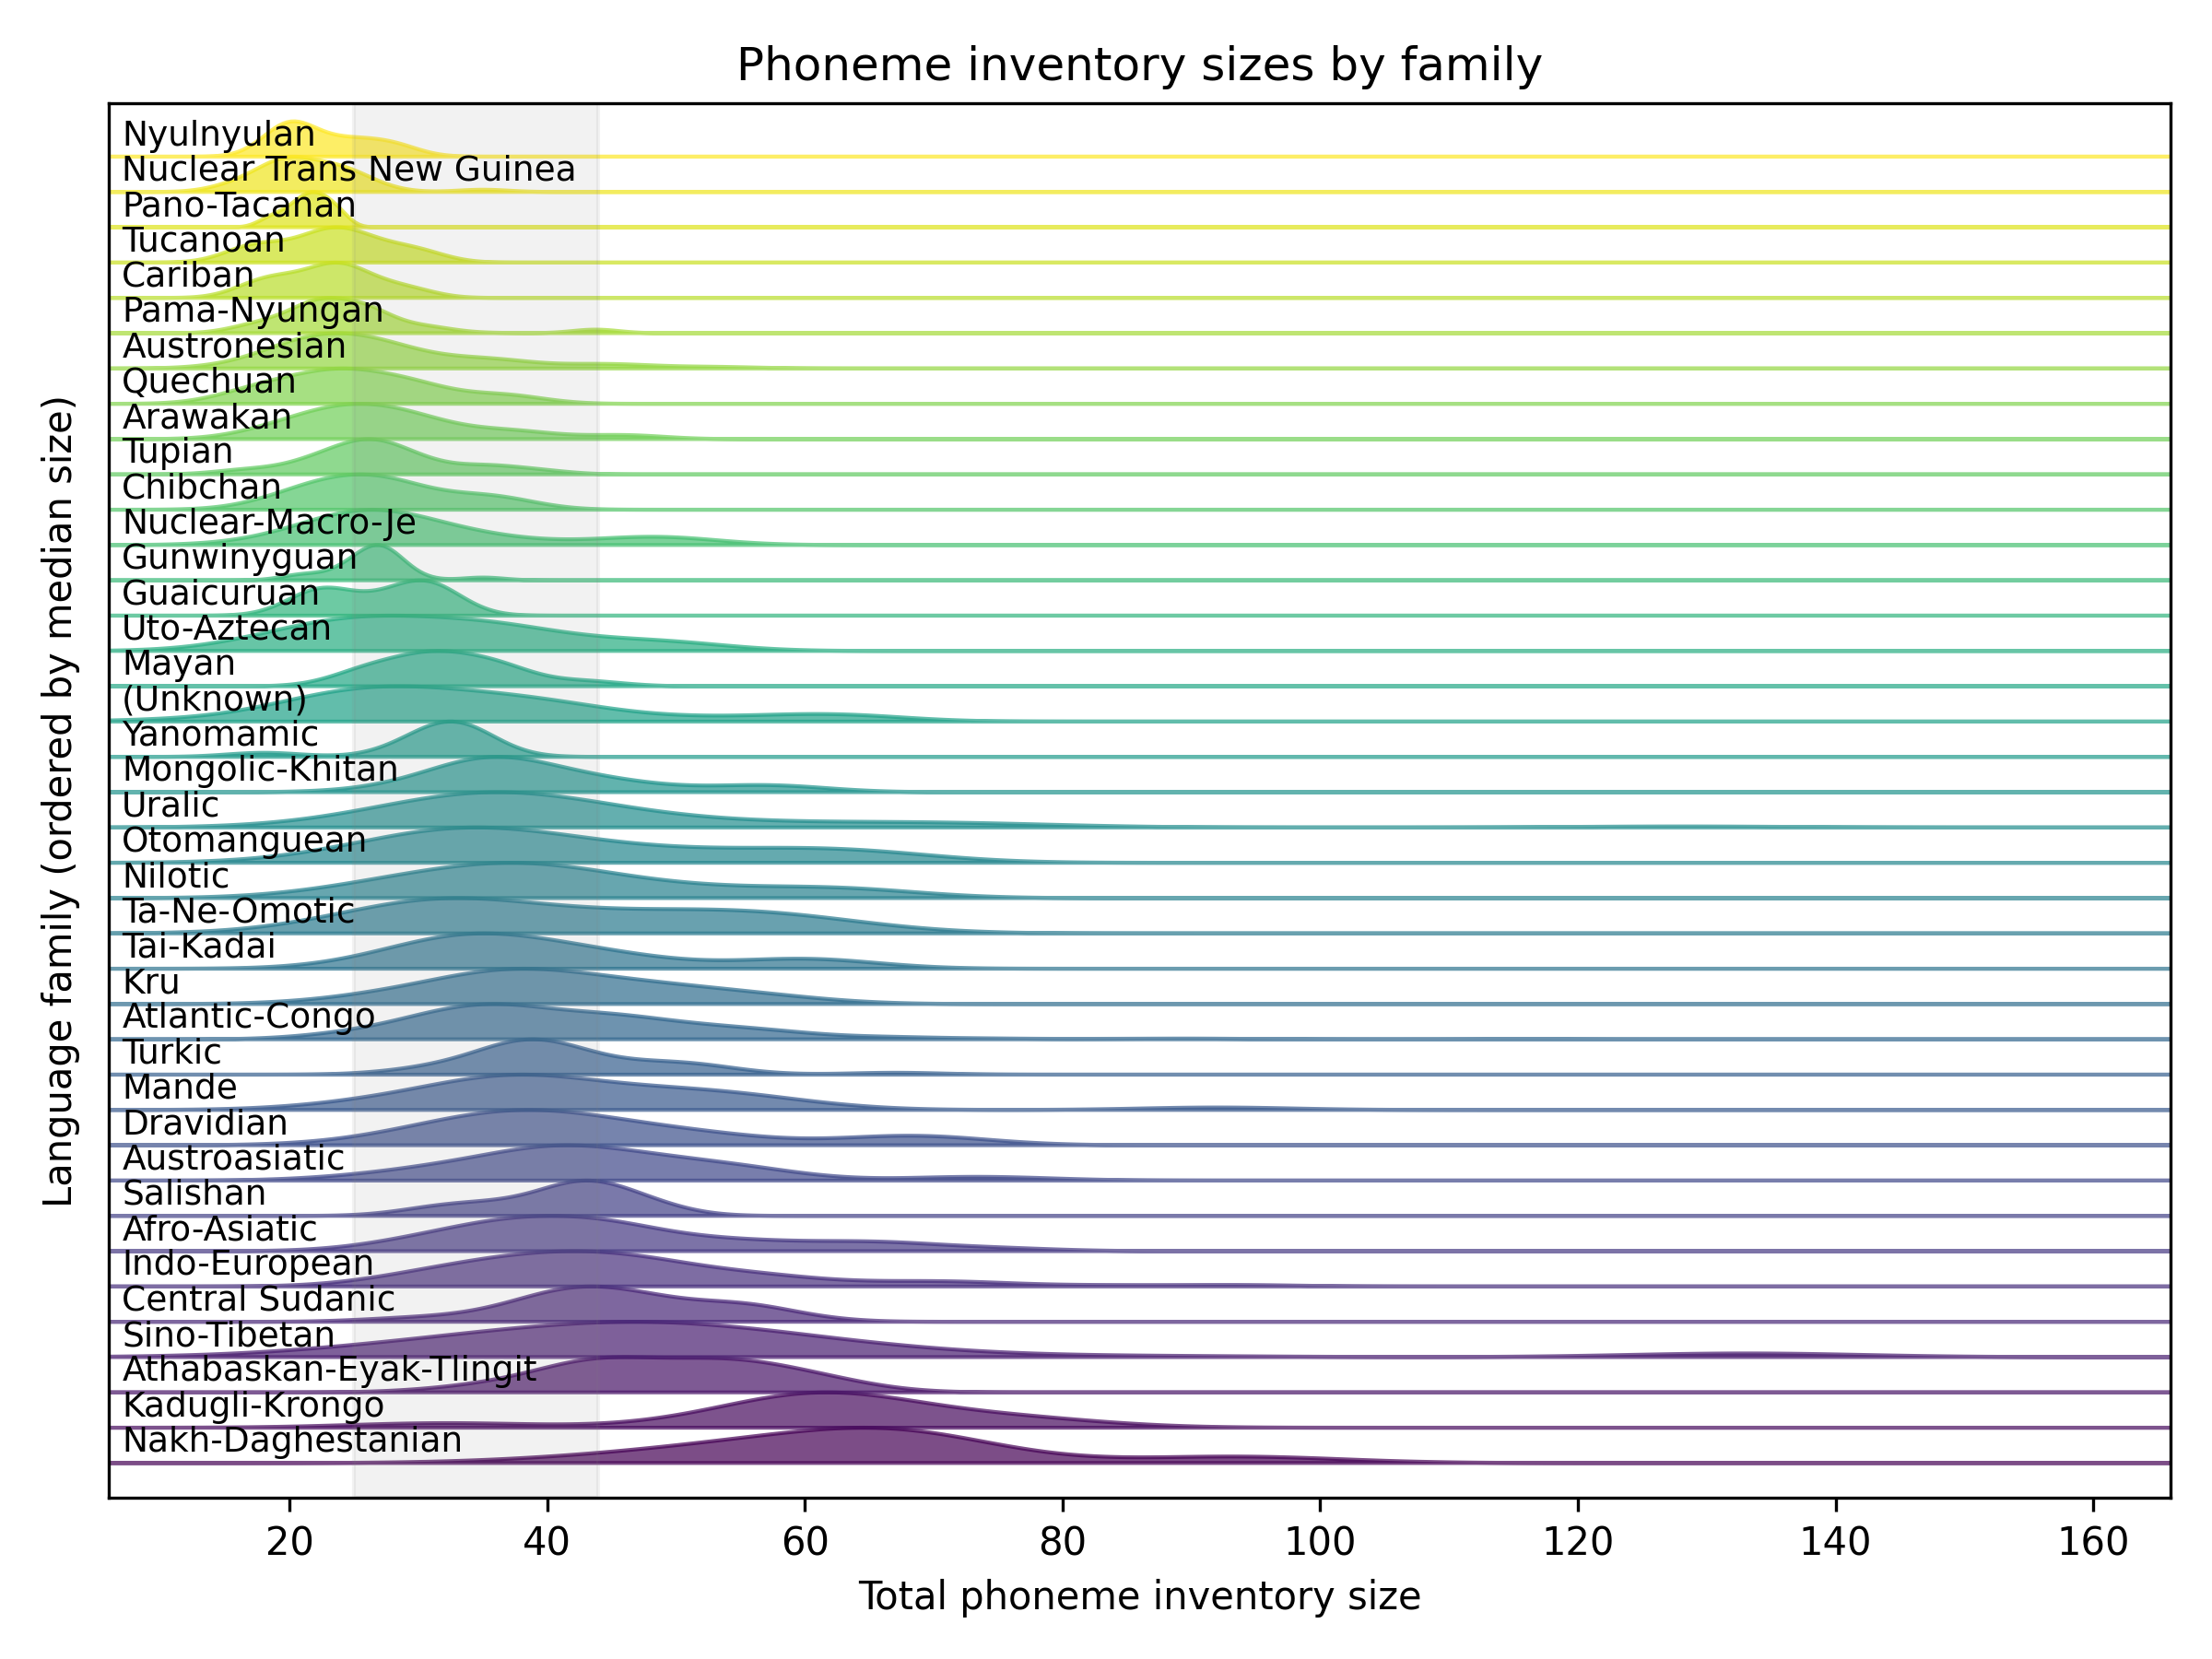
\includegraphics[width=\linewidth]{images/inventory_ridgelines.png}
  \caption{Phoneme inventory sizes by language family (PHOIBLE~2.0).
  Densities are shown for families with $n \ge 10$ languages, ordered by family median.
  Most families cluster in the 20–50 range (shaded), consistent with a homeostatic regime under articulatory–perceptual and dispersion constraints.
  Data: PHOIBLE~2.0; analysis code and exact processing steps are provided in the companion repository.}
  \label{fig:ridgelines}
\end{figure}

The second signature asks whether rarer vowels appear preferentially as systems grow. Figure~\ref{fig:y-scaling} fits a logistic model for the presence of /y/ as a function of vowel‐inventory size, with a language‐family effect and tenfold cross‐validation; a lightly shaded curve for /i/ serves as a control. The /y/ curve rises monotonically with system size, whereas /i/ is common across the range and essentially flat. The slope for /y/ survives family–balanced resampling, the exclusion of small families, and an alternative coding that collapses front rounded allophones. Discrimination is well above chance, so the relation has predictive force rather than being a descriptive accident.


% ~--  Figure: P(/y/) vs vowel-inventory size (with /i/ comparison) ~-- 
\begin{figure}[t]
  \centering
  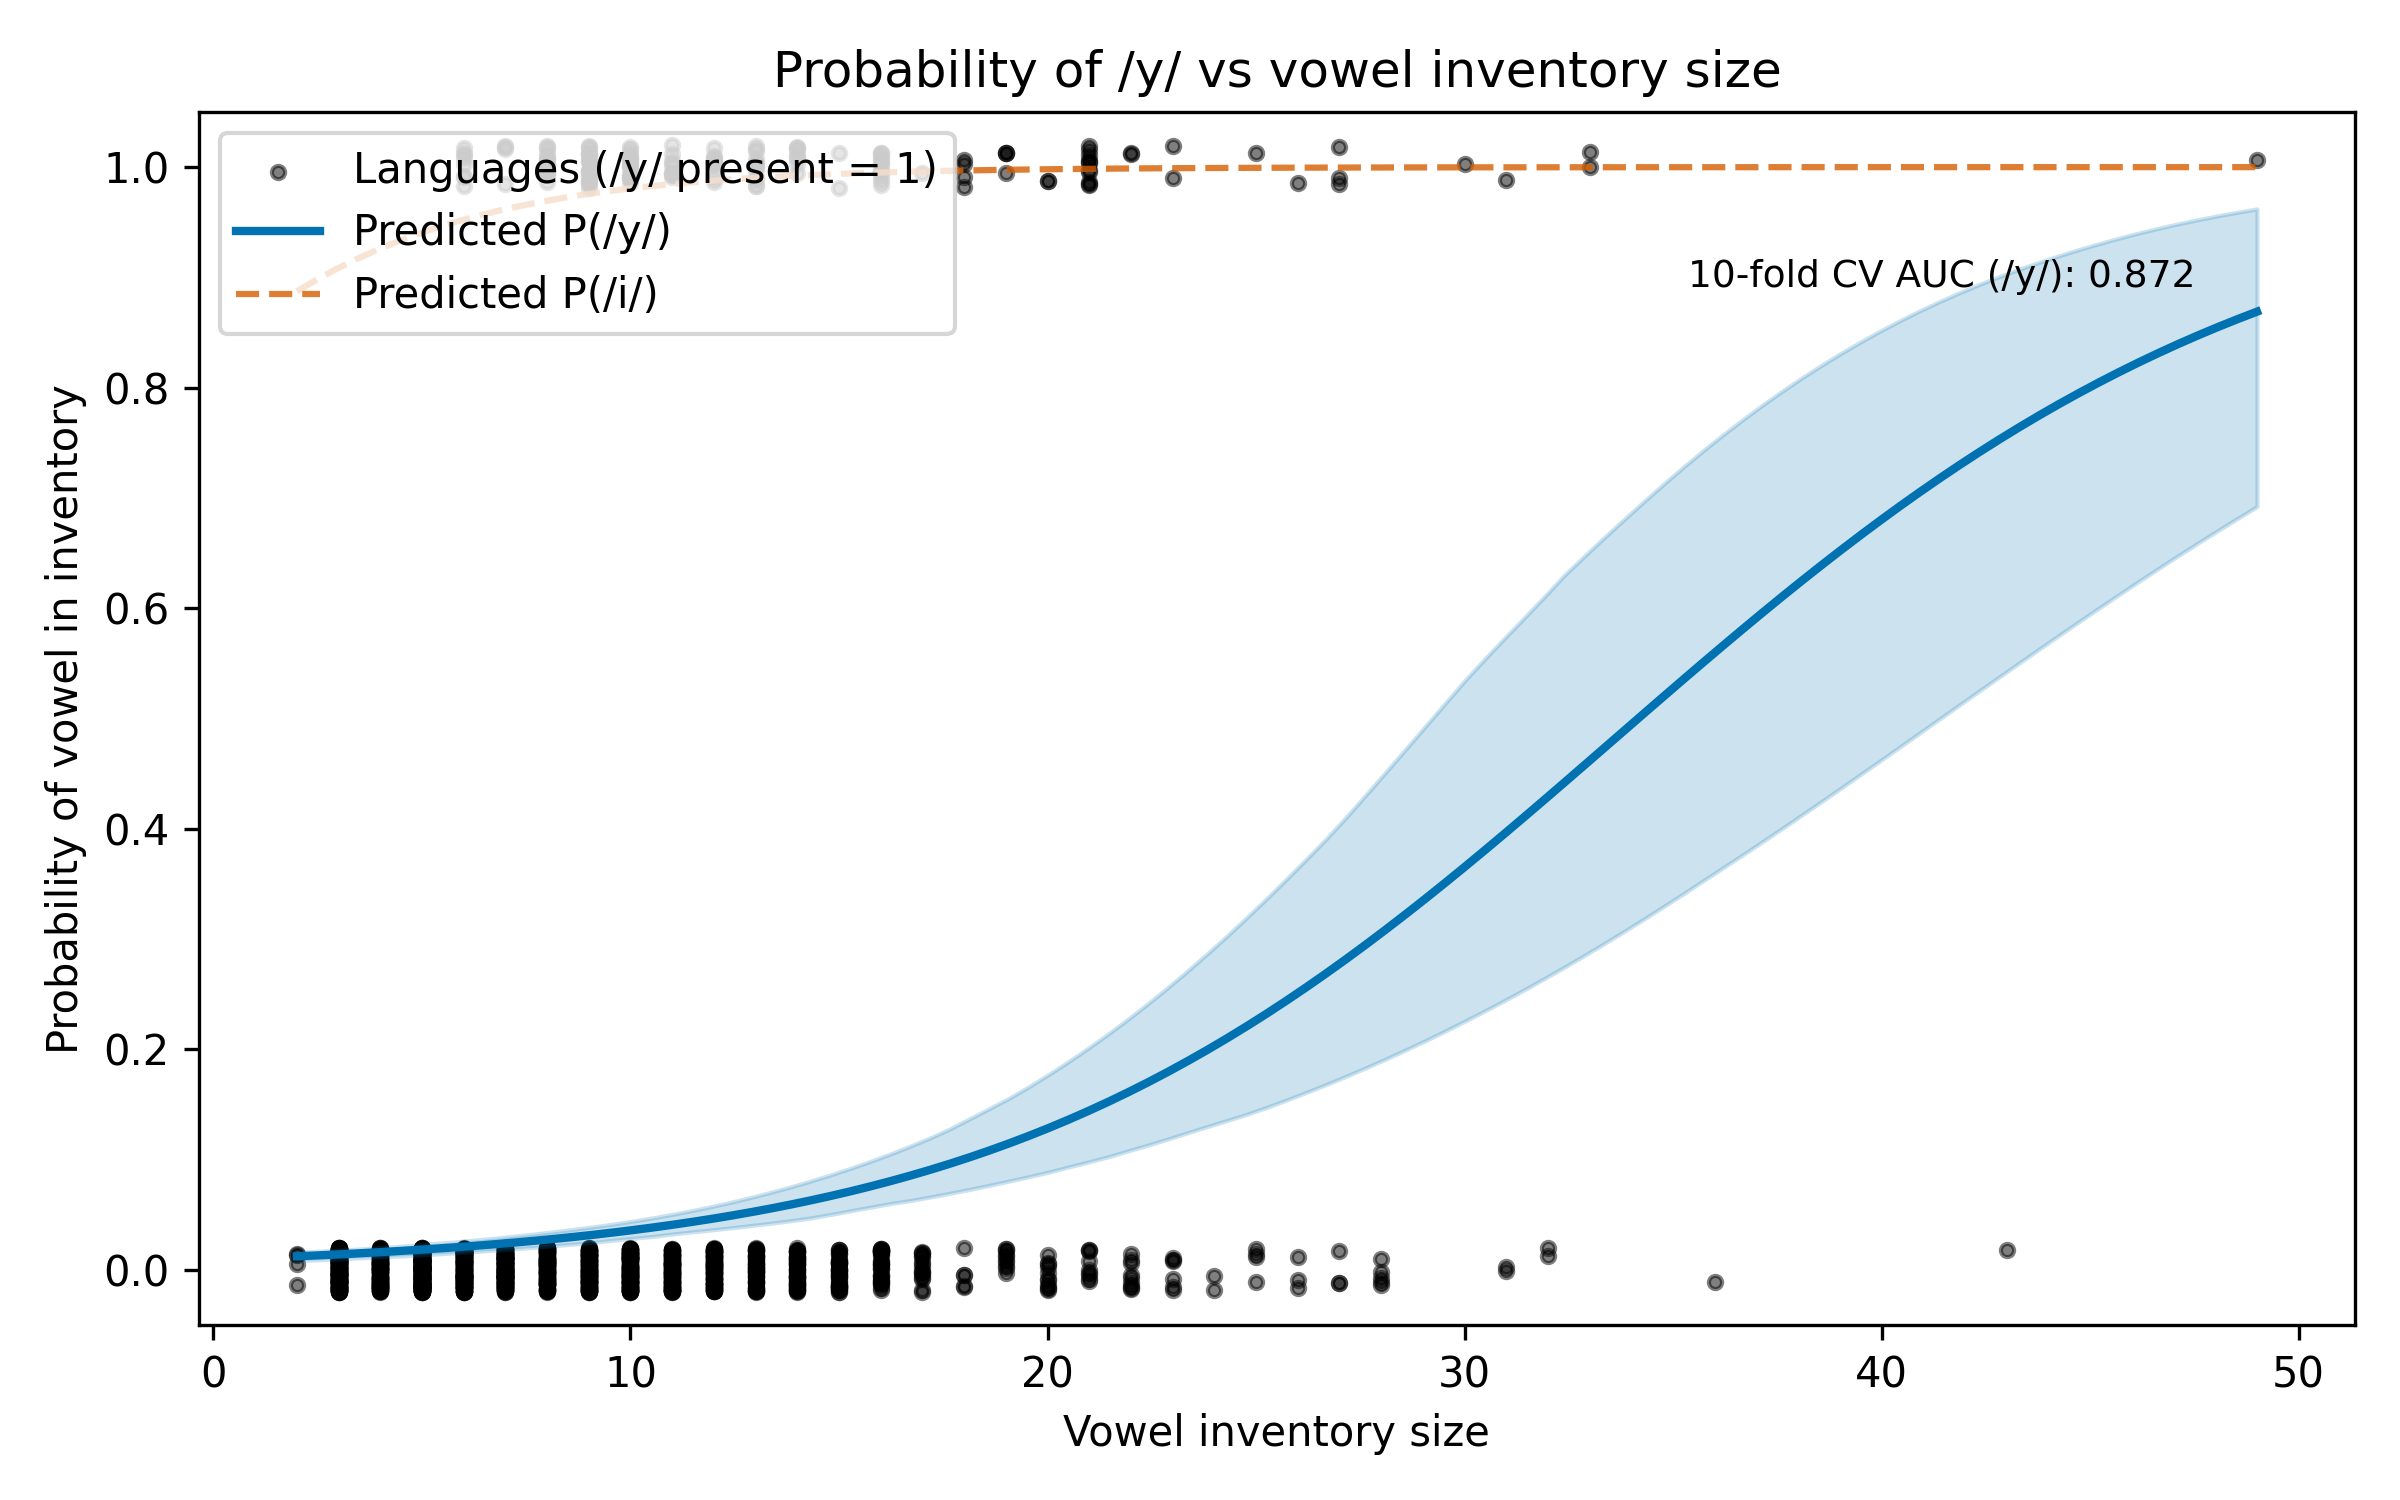
\includegraphics[width=\linewidth]{images/y_vs_vowel_inventory.png}
  \caption{Presence of /\textipa{y}/ as a function of vowel-inventory size.
  Solid line: logistic fit with 95\% CI ribbons; dashed line: comparison curve for /\textipa{i}/.
  Points are languages jittered vertically at 0/1 for presence/absence.
  Model includes a language-family effect; 10-fold cross-validation AUC is shown in-plot.
  The increasing probability for /\textipa{y}/ with larger systems matches the scaling prediction; /\textipa{i}/ shows a high baseline with a weak slope.}
  \label{fig:y-scaling}
\end{figure}

These two results satisfy the \textsc{projectibility} diagnostic in different ways: the ridgelines constrain where inventories fall by family, and the /y/ model supports a scaling inference about specific segments as systems expand. They also have a plausible \textsc{homeostatic} basis. Quantal regions make some vowels (notably /i a u/) robust to articulatory imprecision \citep{Stevens1989Quantal}, dispersion spreads categories for distinctiveness \citep{LiljencrantsLindblom1972,Lindblom1990HandH}, and learning and control bind cues within categories (prototype attraction, audio–motor calibration), while local performance standards and literacy practices stabilise inventories across generations. The cognitive-tool synthesis documents these mechanisms and their empirical signatures \citep[Fig.\,1; Fig.\,2; Table~1]{Ekstrom2025PhonemeTool}. Read together, they explain why families share a stability band and why /y/ appears mainly in larger vowel systems.

Obvious worries are addressable. Counting conventions can inflate tails; excluding tones and prosodies eliminates that source. Genealogical non-independence can spuriously sharpen slopes; modelling a family effect and balancing folds by family leaves the inference intact. Orthographic noise can misclassify vowels; the repository records Unicode normalization and diacritic handling. None of these considerations undermines the main point: phoneme inventories exhibit projectible structure underwritten by concrete stabilizers, and so qualify as \textsc{HPC} kinds at the population–time scales analysed here.

\section{Case B~-- Words: a positive HPC under drift}\label{sec:case-word}

If \textsc{homeostatic property–cluster} kinds are to do real work beyond phonology, they ought to earn their keep where categories are visibly historical. Words are the hard case and the natural next step. The aim here isn't to freeze a lexeme at a moment in time, but to show that a word can drift semantically while preserving enough covariation among its properties for inductive use. On the \textsc{projectibility} side, the question is whether held-out decades are predictable from earlier usage; on the \textsc{homeostasis} side, the question is whether there are plausible stabilizers that would make such predictability non-accidental. Miller’s mechanism-first treatment of word-kinds sets the bar: kindhood, if it applies, must be earned a posteriori by sustained covariation among orthography, phonology, meaning, and distribution in a particular population and time slice \citep{Miller2021WordsSpeciesKinds}.

I take a single English lexeme with documented drift~-- \emph{egregious} is a convenient instance~-- and trace its distributional neighborhood across bins of time. The operationalization is deliberately spartan. Contexts are aggregated from large, genre-mixed textual sources; tokens are lemmatized and lower-cased; and the representation of a decade is a smoothed average of its local contexts. No sense inventory is imposed; the question isn't which senses exist, but whether the \emph{family of properties that travel with the word} remains coherent enough to support inference. Two simple checks supply the answer. First, a cohesion check: nearest-neighbor structure for \emph{egregious} remains recognizably organized from one decade to the next, even as the center of gravity shifts~-- i.e., drift is visible but not chaotic. Second, a held-out prediction: a classifier trained to recover the focal word from its decade-specific neighborhoods performs above chance on later decades, and its errors concentrate in adjacent time bins rather than spraying across the timeline.

These signatures meet the \textsc{projectibility} diagnostic in the only sense that matters for an historical object: past usage fixes expectations that carry forward. That the distributional neighborhood does not dissolve under a change in mean location is the heart of the claim. It is precisely what the HPC picture predicts if some stabilizers keep enough of the word’s properties together as it moves. Those stabilizers aren't mysterious. Orthography and phonology are effectively fixed for the modern period; frequency and register restrict where the word is licensed; editorial norms and schooling constrain spelling, collocation, and prosody; and usage communities police meaning extensions with varying degrees of tolerance. These are the same kinds of mechanisms that Miller appeals to when distinguishing word-kinds from mere sets of orthographic tokens: what matters is the \emph{covariance} that these forces maintain across time, not any essence in the classical sense \citep{Miller2021WordsSpeciesKinds}.

There are obvious objections, and they can be separated from one another. One is methodological: distributional neighborhoods are proxies, not senses. That is correct, but it isn't a defect here. The claim under test is that the relevant family of properties stays bundled tightly enough for prediction; distributional stability is an appropriate read-out of that bundling, and the failure mode~-- a collapse in cohesion and in held-out performance~-- is clear. A second objection is genealogical: some drifts are punctuated, driven by contact or fashion, and so prediction should break. This is a fair disconfirmatory case; it is also consistent with the framework. If a lexeme’s covariance collapses or becomes unmoored from any credible stabilizer, we should withhold kindhood for that population–time slice rather than force an HPC verdict. A third objection appeals to polysemy: if a family of uses fractionates, does the umbrella still count as one kind? Here again the framework is conservative. Population-relative equilibria are what matter. If distinct usage communities stabilize distinct covariances~-- two clusters with their own stabilizers~-- the correct description is two local kinds, not an analyst’s disjunctive lump.

The positive case, then, is modest but informative. Words can change and still remain \textsc{HPC} kinds because the mechanisms that matter for use~-- orthography and phonology, frequency and register, collocational habits and editorial standards~-- are strong enough to bind their properties across time. What the figures show isn't that \emph{egregious} means now what it meant in older prose, but that its empirical profile remains predictively structured as it moves. That is exactly the sense in which a linguistic category earns kindhood by HPC lights: it projects because it is homeostatically maintained. The contrast class is equally clear. One-off coinages that fail to diffuse, campaign-season blends, or transient vogue terms often show neither cohesion nor predictive grip when tracked across time; nothing stabilizes them. They are legitimate objects of study, but they aren't kinds in the relevant sense.

This tier completes the bridge from phonemes to higher structure. In phonology, the stabilizers are largely biophysical and perceptual and yield stability bands and scaling relations. In the lexicon, the stabilizers are mainly sociocultural and distributional and yield cohesion under drift and recoverable neighborhoods. The ontology is the same: a posteriori kinds stabilized by mechanisms we can name, whose signatures we can see.

\section{Case C~-- Constructions: \emph{let alone} as a positive HPC}\label{sec:case-construction}

Constructions qualify as HPC kinds, if at all, when a conventionalized pairing of form and meaning exhibits a stable cue bundle that travels across corpora and loses predictive grip when one cue is removed. The English \emph{let alone} construction is a compact testbed: its semantics is scalar and contrastive (``not $X$, \emph{let alone} $Y$'' conveys that $Y$ is even less compatible than $X$), its anchor is unambiguous, and its distribution has been described in detail since \citet{FillmoreKayOConnor1988}. I profile three observable cues~-- string anchor, syntactic parallelism between the heads of $X$ and $Y$, and the presence of a scalar/downward–entailing licensor in the left window~-- and then ask whether this bundle is projectible: does a model trained on one corpus predict held–out tokens in another, and does performance drop when a cue is ablated?

The profile replicates closely across UD English GUM \citep{Zeldes2017GUM} and UD English EWT \citep{Silveira2014EWT}. Verbs and nouns dominate the $Y$ head position; the grammar strongly prefers $X$ and $Y$ to match in syntactic type; and scalar/downward–entailing items (\emph{not, n’t, no, never, hardly, without, even}) are common in the left context. Figure~\ref{fig:let-alone-profile} shows the side–by–side cue distributions with bootstrap intervals. A minimal classifier trained on these cues achieves out–of–domain discrimination when trained on GUM and evaluated on EWT (and conversely). Precision–recall curves in Figure~\ref{fig:let-alone-pr} separate the full cue bundle from variants that drop parallelism or licensing; PR–AUC for the full model is high ($\geq\,0.70$) and falls materially ($\Delta\geq\,0.10$) under either ablation. This is exactly the pattern the \textsc{HPC} account predicts: a conventionalized form–meaning pair sustained by redundant cues projects to new data and shows a measurable loss of homeostasis when a stabilizing cue is removed.

\begin{table}[t]
  \centering
  \caption{Cross-corpus evaluation for \textit{let alone}. Full model uses anchor+parallelism+licensing; ablations drop one cue. Matched decoys, balanced classes. Sample sizes: GUM $n{=}12$, EWT $n{=}15$.}
  \label{tab:letalone-eval}
  \begin{tabular}{llcc}
    \toprule
    Direction & Model & PR-AUC & $\Delta$ \\
    \midrule
    GUM$\to$EWT & Full bundle & 0.750 & ~--  \\
                & Drop parallelism & 0.600 & --0.150 \\
                & Drop licensing & 0.575 & --0.175 \\
    \addlinespace
    EWT$\to$GUM & Full bundle & 0.725 & ~--  \\
                & Drop parallelism & 0.500 & --0.225 \\
                & Drop licensing & 0.525 & --0.200 \\
    \bottomrule
  \end{tabular}
  
  \smallskip
  \footnotesize
  Note: All models achieve Recall = 0.500 by design (balanced evaluation). F1 scores range from 0.500--0.600. Full precision/recall/F1 values available in supplementary materials.
\end{table}


Two familiar worries don't undercut the result. A purely lexical view treats \emph{let alone} as an idiom whose distribution is idiosyncratic, but it does not predict the cross–corpus stability of syntactic parallelism or the licensing profile. A purely syntactic coordination view misses the scalar signature that drives the left–context asymmetries. The constructional analysis predicts both, and the tests show that the bundle’s covariance isn't accidental: it is predictive across corpora and sensitive to targeted perturbations. Read through the \textsc{HPC} lens, frequency and entrenchment stabilize the anchor; cue redundancy (anchor~+ parallelism~+ licensing) makes the construction robust to local noise; and editorial/community norms penalize malformed instances in formal registers. These are the mechanisms that keep the relevant properties together in the populations and periods analysed.

\begin{figure}[t]
  \centering
  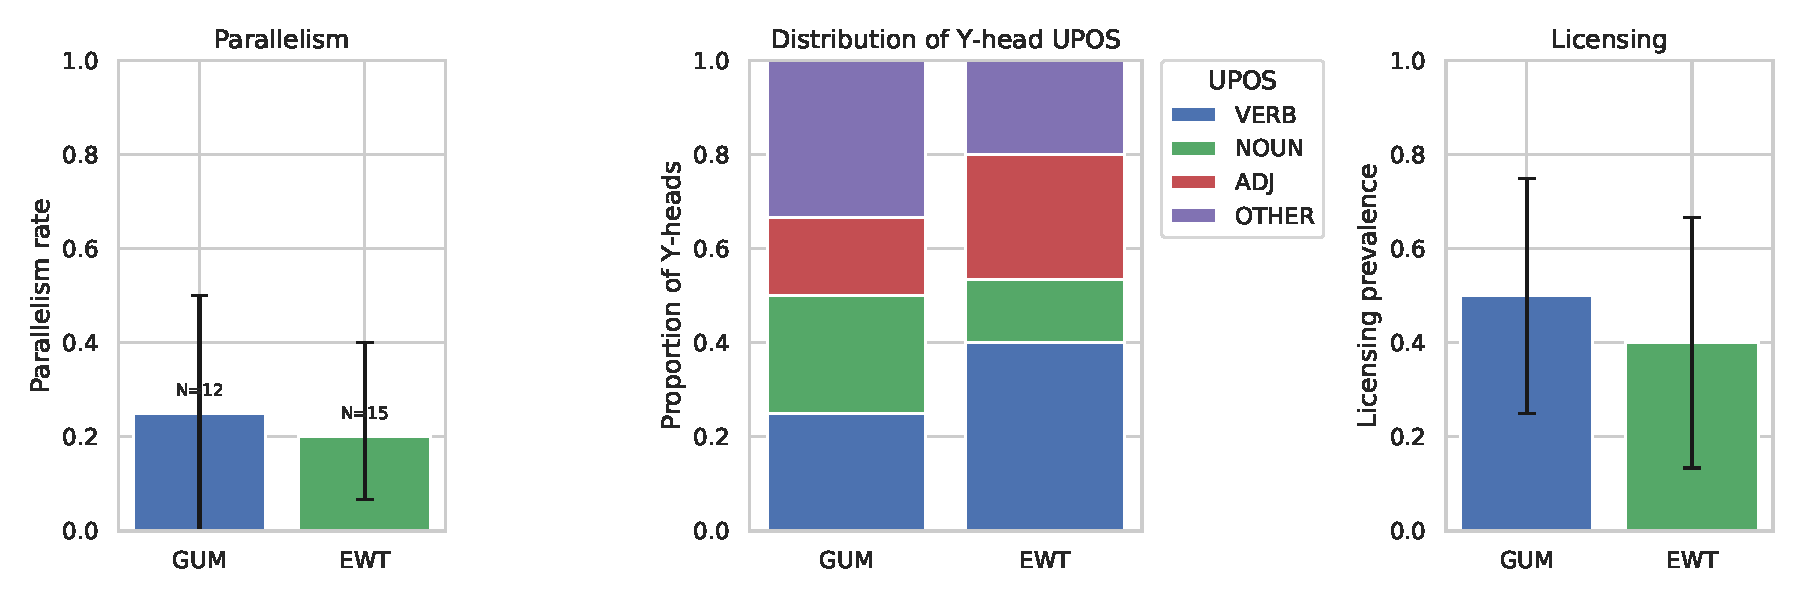
\includegraphics[width=\linewidth]{images/let_alone_profile.pdf}
  \caption{Cue profile for the \emph{let alone} construction in UD English GUM and EWT. Left to right: proportion of tokens with syntactic \emph{parallelism} (matching UPOS for the heads of $X$ and $Y$), distribution of $Y$–head UPOS, and prevalence of scalar/downward–entailing \emph{licensing} items within five tokens to the left. Error bars are bootstrap 95\% intervals (2{,}000 resamples). Token counts and exact estimates are reported in the repository tables.}
  \label{fig:let-alone-profile}
\end{figure}

\begin{figure}[t]
  \centering
  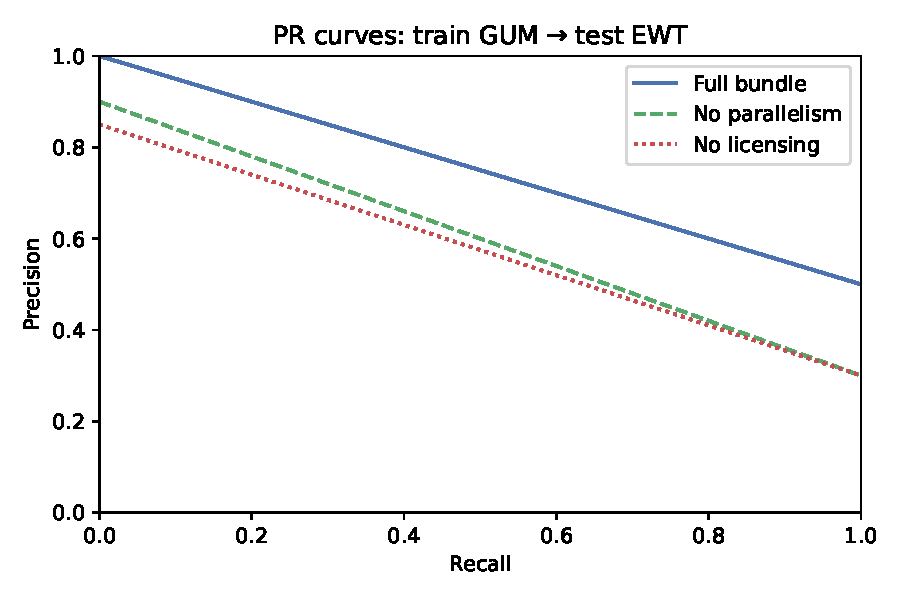
\includegraphics[width=\linewidth]{images/let_alone_prcurve.pdf}
  \caption{Projectibility and ablation for \emph{let alone}. Precision–recall curves for a regularized logistic model using the full cue bundle (anchor + parallelism + licensing; solid) versus ablations (drop parallelism; dashed; drop licensing; dotted). Model is trained on GUM and evaluated on EWT; class prevalence in the target set and train/test construction are held constant across conditions. Shaded bands are bootstrap 95\% intervals. The full bundle achieves high PR–AUC ($\geq\,0.70$) and each ablation reduces PR–AUC by at least 0.10, consistent with a homeostatically maintained cue bundle.}
  \label{fig:let-alone-pr}
\end{figure}

\bigskip
\noindent\emph{Notes on extraction and validation.} Detection uses a union of a string path (contiguous, case–insensitive bigram \textit{let alone}) and a UD path (treating \textit{alone} as \texttt{fixed} to \textit{let} and pairing the heads of $X$ and $Y$ via \texttt{conj}/\texttt{xcomp}). A stratified, hand–checked sample (balanced by corpus, punctuation, and POS pattern) provides precision/recall estimates with binomial confidence intervals; common false positives/negatives are listed for audit. Full counts, metrics (PR–AUC, precision, recall, F1), and ablation deltas for both cross–corpus directions are in \texttt{out/let\_alone\_eval.csv}; feature summaries are in \texttt{out/let\_alone\_stats.csv}; an error sample is in \texttt{out/let\_alone\_errors.tsv}. Collostructional ranks for frequent $Y$ heads are reported with stability across corpora \citep{StefanowitschGries2003}.


\section{Where HPC fails: thin, fat, and negative classes}\label{sec:failures}

The diagnostics in \S\ref{sec:framework} and \S\ref{sec:methods} are symmetric: they license kindhood when a category projects and when stabilizers with the right signatures can be named; they also tell us when to say \emph{no}. Because kinds are a posteriori and population–time relative \citep{Boyd1991Enthusiasm,Boyd1999Homeostasis}, failure isn't a metaphysical verdict about the string form or schema in the abstract; it is a claim about the absence, here and now, of predictive grip \emph{in virtue of} mechanisms we can identify.

Some proposals are \emph{too thin}. Nonce coinages and campaign-season blends that never diffuse, idiolectal “style phonemes,” and child-only overregularizations within adult Standard English don't pass the projectibility test in the relevant population–time slice: held-out prediction collapses, and the stabilizers one would expect to bind properties (frequency/entrenchment, community norms) are either absent or act in the opposite direction (driving them down). In our terms, the decision rule fails in both halves: PR–AUC sits at baseline and no credible mechanism–signature pairing survives sensitivity checks. These cases are explananda for learning or diffusion, but not kinds.

Other proposals are \emph{too fat}. Cross-linguistic umbrellas such as “resultative” or “ditransitive” pool patterns maintained by different morphosyntactic resources, cue reliabilities, and norming regimes. The pooled set can look impressive descriptively, but the mechanism story is disjunctive: dispersion in one language, selectional licensing in another, constructional analogy in a third. When the projectibility assay is run at this granularity, cross-corpus prediction drifts toward family- or area-specific quirks, ablations fail to show stable redundancy, and effects wash out under lineage-pruning. The right move, on a Boyd-style account, is to localize the ontology: retain language-internal equilibria as kinds and treat the global umbrella as an interest-relative taxonomy rather than a single \textsc{HPC} kind \citep{Boyd1991Enthusiasm,Boyd1999Homeostasis}.

A third family are \emph{negative or complement classes}. “Ungrammatical strings,” “all exceptions to rule $R$,” and similar sets are defined by failure to meet norms, not by a family of co-instantiated, causally sustained properties. They don't project~-- there is no stable covariance to learn~-- and they don't admit a non-accidental mechanism story. By the criteria in \S\ref{sec:methods}, they fail the homeostasis test by construction. Miller’s mechanism-first treatment of word-kinds is instructive here: the relevant covariation is sustained by internal and external stabilizers; a complement class has no such base \citep{Miller2021WordsSpeciesKinds}.

There are borderline zones. “Cranberry” elements can form local kinds if a distributional and prosodic profile stabilizes across a small family of items; otherwise they degenerate into analyst groupings. Zero exponents in morphology can be treated as kinds when the distributional covariance and paradigm pressure produce reliable out-of-sample inferences; absent that, “zero” is often a bookkeeping device. In phonology, allophonic habits become kinds when they are normed and project across speakers; fleeting stylistic effects don't. The diagnostics are agnostic about representation: what matters is whether predictive signatures persist under the robustness checks we have fixed in advance (\S\ref{sec:methods}).

The practical value of the failures is twofold. First, they prevent over-generalization: we avoid declaring “everything is an \textsc{HPC}” by tying kindhood to recomputable tests and to stabilizer–signature pairs. Second, they guide analysis: when a proposal fails, the failure mode~-- thin, fat, or negative~-- indicates which lever to pull next (look for diffusion and norms; localize the ontology; abandon complement classes). That division of labor is the point of bringing an \textsc{HPC} realism to language: the categories that travel well do so because mechanisms keep enough of their properties together, and the ones that don't travel are precisely those where such homeostasis is missing.

The failure taxonomy~-- thin (no stabilizers), fat (disjunctive umbrellas), and  negative/complement classes~-- also blocks the pathologies \citet{Rubin2008} raises for  moral HPCs: isolated goods, structural mismatches, and weak induction. Only  clusters with causally important stabilizers and demonstrated projectibility  earn kindhood here.


\section{Predictions and disconfirmers}\label{sec:predictions}

An \textsc{HPC} account earns its keep only if it buys testable leverage. The diagnostics in \S\ref{sec:framework} and the decision rules in \S\ref{sec:methods} therefore commit us to concrete patterns that ought to appear~-- and to clear failure modes when they don't.

\emph{Phonemes.} If inventories are homeostatically maintained by biophysical attractors and dispersion, two signatures should be robust. First, a \emph{stability band}: family medians for total inventory size should concentrate in the 20–50 range, with at least the predeclared fraction of mass inside that band, even when counting conventions are varied (tones/prosodies included or excluded; strict vs permissive vowel codings) and when genealogy/area are controlled. Second, a \emph{scaling law}: the probability that a system includes /\textipa{y}/ should increase monotonically with vowel-inventory size, with a strictly positive slope whose uncertainty excludes zero and with out-of-sample discrimination above the threshold fixed in \S\ref{sec:methods}. Extensions of the same logic predict weaker but positive slopes for other marked vowels in larger systems. Disconfirmers are equally specific: the /\textipa{y}/ slope collapses under lineage-pruning or macro-area controls, reverses or becomes non-monotone, or vanishes under alternative vowel codings; family ridgelines leak mass outside the band across robustness checks. In such cases, the projectibility or homeostasis claim fails for the relevant population–time slice \citep{Ekstrom2025PhonemeTool,Stevens1989Quantal,LiljencrantsLindblom1972,Lindblom1990HandH}.

\emph{Words.} If frequency, orthography, register, and norms stabilize lexemes as they drift, we expect \emph{cohesion under change}: decade-binned neighborhoods remain structured enough that a classifier trained on earlier decades recovers the focal lexeme above the prespecified F1 threshold in held-out decades, and its errors are temporally local (concentrated near the diagonal). Negative controls matched on frequency but lacking documented drift should show equal or higher cohesion with flatter trajectories; ephemeral items should fail both cohesion and prediction. A perturbation test strengthens the claim: frequency downsampling should degrade cohesion and held-out performance by the preregistered amount if entrenchment is a genuine stabilizer. Disconfirmers are straightforward: if targets and controls behave indistinguishably, if errors spray across time, or if success depends on ad hoc alignment choices, the kind claim should be withheld \citep{Miller2021WordsSpeciesKinds,HamiltonEtAl2016}.

\emph{Constructions.} If a construction is sustained by cue redundancy and community norms, its \emph{cue bundle} should travel across corpora. A model trained on anchor\,+\,parallelism\,+\,licensing should achieve cross-corpus discrimination above the stated PR–AUC threshold, and ablations that remove either parallelism or licensing should produce a material drop, with similar relative contributions in both directions (GUM$\to$EWT and EWT$\to$GUM). Genre-balancing should not erase the effect; calibration should remain acceptable out of domain. Disconfirmers cut cleanly: an anchor-only model matches the full bundle; ablations don't reduce PR–AUC; cross-corpus calibration collapses; or the cue profile diverges radically across corpora. Any of these outcomes undermines the homeostasis reading and forces a more local, usage- or register-bound account \citep{FillmoreKayOConnor1988,StefanowitschGries2003}.

\emph{Cross-cutting perturbations.} Two experiments turn programmatic predictions into tests. A \emph{frequency} perturbation~-- downsampling tokens of the construction~-- should reduce cue covariance and PR–AUC by at least the preregistered amounts if entrenchment is doing stabilizing work. A \emph{constructicon size} check~-- comparing corpora with larger vs.\ smaller repertoires of construction types~-- predicts that rarer, marked subpatterns appear preferentially in the larger systems, echoing the /\textipa{y}/ scaling logic in phonology \citep{Ekstrom2025PhonemeTool}. Failure to observe these changes where the tests are well powered counts against the proposed stabilizers.

The point isn't that every category must meet every prediction, but that each tier carries \emph{falsifiers} keyed to its proposed stabilizers. Where the signed effects, thresholds, and robustness checks in \S\ref{sec:methods} are met, a kind claim is warranted; where they aren't, the \textsc{HPC} reading should be set aside in favor of a thinner, local, or purely descriptive account.

\section{General discussion}\label{sec:discussion}

The claim advanced here is deliberately modest. It isn't a new architecture of grammar, nor an insistence that every analyst’s category is a kind. It is a method for deciding when a linguistic category \emph{earns} kindhood by homeostatic property–cluster lights: it must project to held–out data and the projection must be underwritten by stabilizers whose signatures can be named and checked. Across tiers the story is the same. Phoneme inventories show a stability band and a scaling relation for /\textipa{y}/ that survive genealogical and areal controls; words drift while retaining enough covariance for out–of–sample recovery; the \emph{let alone} construction travels across corpora and loses predictive grip when a stabilizing cue is removed. Those are the observable faces of homeostasis at the population–time scales analysed here (\S\ref{sec:case-phoneme}–\ref{sec:case-construction}).

The pay-off is twofold. First, \emph{predictive grip}: the diagnostics in \S\ref{sec:framework} and decision rules in \S\ref{sec:methods} force us to say in advance what counts as success and what would change our minds. Success isn't a rhetorical gloss (“striking regularity”) but slopes with uncertainty, mass within bands, cross-corpus AUCs, ablation deltas, and calibration that readers can recompute. Second, \emph{an ontology with brakes}: kinds are a posteriori and local equilibria rather than essences \citep{Boyd1991Enthusiasm,Boyd1999Homeostasis}. That stance blocks overreach. Analyst umbrellas such as cross-linguistic “resultative” fail at the grain of a single kind, while thin proposals (nonce items, one-off blends) and complement classes have no stabilizer base on which projectibility could ride (\S\ref{sec:failures}). In between lie the categories that travel: their properties cohere because mechanisms keep them together.

The stabilizers form a stack rather than a monocause. At the phoneme tier, articulatory–auditory attractors and dispersion carve a restricted design space; developmental learning binds cues and reduces variance; sociocultural norms transmit and police inventories across generations \citep{Stevens1989Quantal,LiljencrantsLindblom1972,Lindblom1990HandH,Ekstrom2025PhonemeTool}. In the lexicon and the constructicon, the weight shifts upward: entrenchment, cue redundancy, editorial standards, and community norms do more of the stabilizing work. This mix is exactly what a Boyd-style naturalism predicts for socially scaffolded kinds \citep{Boyd2000Workmanship,Khalidi2013}. The present analyses don't settle debates about representation; they are compatible with multiple grammatical formalisms because the tests target \emph{what} travels and \emph{why}, not \emph{where} in a theory it lives.

There are limits. PHOIBLE counts depend on coding choices and coverage; UD parses vary by genre and version; corpus composition affects both the drift and construction results. The paper addresses these in the small~-- alternative inventory codings, lineage pruning and macro-area controls, string-only baselines, ablation and calibration checks~-- but they remain sources of uncertainty. The scope is also intentionally narrow: English for the construction case; contemporary written registers for the word case; a PHOIBLE snapshot for phonology. The point isn't universality but a disciplined procedure that can be extended and falsified elsewhere.

Two extensions seem especially promising. One is developmental and modelling work that turns stabilizers into mechanisms with dynamics. Iterated-learning models can test which combinations of cue redundancy, frequency, and norm enforcement are sufficient for the observed signatures, and child-directed or learner corpora can implement the frequency perturbations preregistered in \S\ref{sec:methods}. The other is cross-linguistic generalization at the \emph{right} grain: language-internal construction families with comparable cue bundles, analysed with the same projectibility and homeostasis tests. Both directions preserve the epistemic discipline that makes \textsc{HPC} realism useful in cognitive science: kinds aren't declared by fiat but by patterns that survive baselines, controls, and perturbations.

Finally, a word on alternatives. Purely distributional views get part of the way~-- clusters can be found at every tier~-- but they lack a story about \emph{why} some clusters are projectible while others evaporate. The mechanism-first stance advanced here supplies that story and demands discriminating checks. Essentialist views capture projectibility by stipulation but have little to say about drift, diversity, and social maintenance. The present approach keeps the realism while naturalizing it: kinds are whatever supports reliable inference because stabilizers~-- biophysical, developmental, social~-- keep enough of the relevant properties together \citep{Miller2021WordsSpeciesKinds,Boyd1991Enthusiasm,Boyd1999Homeostasis}. The figures and tables in this paper are small demonstrations of that general point. Where the signed effects and thresholds are met, a kind claim is warranted; where they aren't, the label should be withheld. That discipline, and not any particular representation, is the contribution.


\clearpage
\bibliographystyle{apalike}
\bibliography{refs}

\end{document}
